% Created 2022-01-23 Sun 13:16
% Intended LaTeX compiler: pdflatex
\documentclass{scrartcl}
\renewcommand\sectionformat{\llap{\thesection\autodot\enskip}}
\renewcommand\subsectionformat{\llap{\thesubsection\autodot\enskip}}
\renewcommand\subsubsectionformat{\llap{\thesubsubsection\autodot\enskip}}

\usepackage[utf8]{inputenc}
\usepackage[T1]{fontenc}
\usepackage{fontspec}
\usepackage{xcolor}
\usepackage{hyperref}
\usepackage{firamath-otf}
\setmonofont{Liga SFMono Nerd Font}
\setmainfont{Fira Sans}
% features: (acronym underline italic-quotes par-sep condensed-lists image caption cover-page)
\newcommand{\acr}[1]{\protect\textls*[110]{\scshape #1}}
\newcommand{\acrs}{\protect\scalebox{.91}[.84]{\hspace{0.15ex}s}}
\usepackage[normalem]{ulem}
\renewcommand{\quote}{\list{}{\rightmargin\leftmargin}\item\relax\em}

\setlength{\parskip}{\baselineskip}
\setlength{\parindent}{0pt}


\newcommand{\setuplistspacing}{\setlength{\itemsep}{-0.5ex}\setlength{\parskip}{1.5ex}\setlength{\parsep}{0pt}}
\let\olditem\itemize\renewcommand{\itemize}{\olditem\setuplistspacing}
\let\oldenum\enumerate\renewcommand{\enumerate}{\oldenum\setuplistspacing}
\let\olddesc\description\renewcommand{\description}{\olddesc\setuplistspacing}
   
\usepackage{graphicx}

\usepackage{subcaption}
\usepackage[hypcap=true]{caption}
\setkomafont{caption}{\sffamily\small}
\setkomafont{captionlabel}{\upshape\bfseries}
\captionsetup{justification=raggedright,singlelinecheck=true}
\usepackage{capt-of} % required by Org


\usepackage{tikz}
\usetikzlibrary{shapes.geometric}
\usetikzlibrary{calc}

\newsavebox\orgicon
\begin{lrbox}{\orgicon}
  
\begin{tikzpicture}[y=0.80pt, x=0.80pt, inner sep=0pt, outer sep=0pt]
    \path[fill=black!6] (16.15,24.00) .. controls (15.58,24.00) and (13.99,20.69) .. (12.77,18.06)arc(215.55:180.20:2.19) .. controls (12.33,19.91) and (11.27,19.09) .. (11.43,18.05) .. controls (11.36,18.09) and (10.17,17.83) .. (10.17,17.82) .. controls (9.94,18.75) and (9.37,19.44) .. (9.02,18.39) .. controls (8.32,16.72) and (8.14,15.40) .. (9.13,13.80) .. controls (8.22,9.74) and (2.18,7.75) .. (2.81,4.47) .. controls (2.99,4.47) and (4.45,0.99) .. (9.15,2.41) .. controls (14.71,3.99) and (17.77,0.30) .. (18.13,0.04) .. controls (18.65,-0.49) and (16.78,4.61) .. (12.83,6.90) .. controls (10.49,8.18) and (11.96,10.38) .. (12.12,11.15) .. controls (12.12,11.15) and (14.00,9.84) .. (15.36,11.85) .. controls (16.58,11.53) and (17.40,12.07) .. (18.46,11.69) .. controls (19.10,11.41) and (21.79,11.58) .. (20.79,13.08) .. controls (20.79,13.08) and (21.71,13.90) .. (21.80,13.99) .. controls (21.97,14.75) and (21.59,14.91) .. (21.47,15.12) .. controls (21.44,15.60) and (21.04,15.79) .. (20.55,15.44) .. controls (19.45,15.64) and (18.36,15.55) .. (17.83,15.59) .. controls (16.65,15.76) and (15.67,16.38) .. (15.67,16.38) .. controls (15.40,17.19) and (14.82,17.01) .. (14.09,17.32) .. controls (14.70,18.69) and (14.76,19.32) .. (15.50,21.32) .. controls (15.76,22.37) and (16.54,24.00) .. (16.15,24.00) -- cycle(7.83,16.74) .. controls (6.83,15.71) and (5.72,15.70) .. (4.05,15.42) .. controls (2.75,15.19) and (0.39,12.97) .. (0.02,10.68) .. controls (-0.02,10.07) and (-0.06,8.50) .. (0.45,7.18) .. controls (0.94,6.05) and (1.27,5.45) .. (2.29,4.85) .. controls (1.41,8.02) and (7.59,10.18) .. (8.55,13.80) -- (8.55,13.80) .. controls (7.73,15.00) and (7.80,15.64) .. (7.83,16.74) -- cycle;
  \end{tikzpicture}
\end{lrbox}

\makeatletter
\g@addto@macro\tableofcontents{\clearpage}
\renewcommand\maketitle{
  \thispagestyle{empty}
  \hyphenpenalty=10000 % hyphens look bad in titles
  \renewcommand{\baselinestretch}{1.1}
  \let\oldtoday\today
  \renewcommand{\today}{\LARGE\number\year\\\large%
    \ifcase \month \or Jan\or Feb\or Mar\or Apr\or May \or Jun\or Jul\or Aug\or Sep\or Oct\or Nov\or Dec\fi
    ~\number\day}
  
\begin{tikzpicture}[remember picture,overlay]
    %% Background Polygons %%
    \foreach \i in {2.5,...,22} % bottom left
    {\node[rounded corners,black!3.5,draw,regular polygon,regular polygon sides=6, minimum size=\i cm,ultra thick] at ($(current page.west)+(2.5,-4.2)$) {} ;}
    \foreach \i in {0.5,...,22} % top left
    {\node[rounded corners,black!5,draw,regular polygon,regular polygon sides=6, minimum size=\i cm,ultra thick] at ($(current page.north west)+(2.5,2)$) {} ;}
    \node[rounded corners,fill=black!4,regular polygon,regular polygon sides=6, minimum size=5.5 cm,ultra thick] at ($(current page.north west)+(2.5,2)$) {};
    \foreach \i in {0.5,...,24} % top right
    {\node[rounded corners,black!2,draw,regular polygon,regular polygon sides=6, minimum size=\i cm,ultra thick] at ($(current page.north east)+(0,-8.5)$) {} ;}
    \node[fill=black!3,rounded corners,regular polygon,regular polygon sides=6, minimum size=2.5 cm,ultra thick] at ($(current page.north east)+(0,-8.5)$) {};
    \foreach \i in {21,...,3} % bottom right
    {\node[black!3,rounded corners,draw,regular polygon,regular polygon sides=6, minimum size=\i cm,ultra thick] at ($(current page.south east)+(-1.5,0.75)$) {} ;}
    \node[fill=black!3,rounded corners,regular polygon,regular polygon sides=6, minimum size=2 cm,ultra thick] at ($(current page.south east)+(-1.5,0.75)$) {};
    \node[align=center, scale=1.4] at ($(current page.south east)+(-1.5,0.75)$) {\usebox\orgicon};
    %% Text %%
    \node[left, align=right, black, text width=0.8\paperwidth, minimum height=3cm, rounded corners,font=\Huge\bfseries] at ($(current page.north east)+(-2,-8.5)$)
    {\@title};
    \node[left, align=right, black, text width=0.8\paperwidth, minimum height=2cm, rounded corners, font=\Large] at ($(current page.north east)+(-2,-11.8)$)
    {\scshape \@author};
    \renewcommand{\baselinestretch}{0.75}
    \node[align=center,rounded corners,fill=black!3,text=black,regular polygon,regular polygon sides=6, minimum size=2.5 cm,inner sep=0, font=\Large\bfseries ] at ($(current page.west)+(2.5,-4.2)$)
    {\@date};
  \end{tikzpicture}
  \let\today\oldtoday
  \clearpage}
\makeatother
   
% end features

%% make document follow Emacs theme

\definecolor{obg}{HTML}{FFFFFF}
\definecolor{ofg}{HTML}{37474F}

\pagecolor{obg}
\color{ofg}

% list labels

\definecolor{itemlabel}{HTML}{B0BEC5}

\renewcommand{\labelitemi}{\textcolor{itemlabel}{\textbullet}}
\renewcommand{\labelitemii}{\textcolor{itemlabel}{\normalfont\bfseries \textendash}}
\renewcommand{\labelitemiii}{\textcolor{itemlabel}{\textasteriskcentered}}
\renewcommand{\labelitemiv}{\textcolor{itemlabel}{\textperiodcentered}}

\renewcommand{\labelenumi}{\textcolor{itemlabel}{\theenumi.}}
\renewcommand{\labelenumii}{\textcolor{itemlabel}{(\theenumii)}}
\renewcommand{\labelenumiii}{\textcolor{itemlabel}{\theenumiii.}}
\renewcommand{\labelenumiv}{\textcolor{itemlabel}{\theenumiv.}}

% structural elements

\definecolor{documentTitle}{HTML}{B0BEC5}
\definecolor{documentInfo}{HTML}{B0BEC5}
\definecolor{level1}{HTML}{263238}
\definecolor{level2}{HTML}{263238}
\definecolor{level3}{HTML}{263238}
\definecolor{level4}{HTML}{263238}
\definecolor{level5}{HTML}{263238}
\definecolor{level6}{HTML}{263238}
\definecolor{level7}{HTML}{263238}
\definecolor{level8}{HTML}{263238}

\addtokomafont{title}{\color{documentTitle}}
\addtokomafont{author}{\color{documentInfo}}
\addtokomafont{date}{\color{documentInfo}}
\addtokomafont{section}{\color{level1}}
\newkomafont{sectionprefix}{\color{level1}}
\addtokomafont{subsection}{\color{level2}}
\newkomafont{subsectionprefix}{\color{level2}}
\addtokomafont{subsubsection}{\color{level3}}
\newkomafont{subsubsectionprefix}{\color{level3}}
\addtokomafont{paragraph}{\color{level4}}
\newkomafont{paragraphprefix}{\color{level4}}
\addtokomafont{subparagraph}{\color{level5}}
\newkomafont{subparagraphprefix}{\color{level5}}

% textual elements

\definecolor{link}{HTML}{673AB7}
\definecolor{cite}{HTML}{673AB7}
\definecolor{itemlabel}{HTML}{B0BEC5}
\definecolor{code}{HTML}{B0BEC5}
\definecolor{verbatim}{HTML}{FFAB91}

\renewcommand{\labelitemi}{\textcolor{itemlabel}{\textbullet}}
\renewcommand{\labelitemii}{\textcolor{itemlabel}{\normalfont\bfseries \textendash}}
\renewcommand{\labelitemiii}{\textcolor{itemlabel}{\textasteriskcentered}}
\renewcommand{\labelitemiv}{\textcolor{itemlabel}{\textperiodcentered}}

\renewcommand{\labelenumi}{\textcolor{itemlabel}{\theenumi.}}
\renewcommand{\labelenumii}{\textcolor{itemlabel}{(\theenumii)}}
\renewcommand{\labelenumiii}{\textcolor{itemlabel}{\theenumiii.}}
\renewcommand{\labelenumiv}{\textcolor{itemlabel}{\theenumiv.}}

\DeclareTextFontCommand{\texttt}{\color{code}\ttfamily}
\makeatletter
\def\verbatim@font{\color{verbatim}\normalfont\ttfamily}
\makeatother

% code blocks

\definecolor{codebackground}{HTML}{FFFFFF}
\colorlet{EFD}{ofg}
\definecolor{codeborder}{HTML}{B0BEC5}

%% end customisations

\author{Shaurya Singh}
\date{\today}
\title{Accelerating Precision Medicine with Quantum Computing and AI\\\bigskip
\LARGE\mdseries\itshape\color{black!80} Exploring the future of Personalized Health Care\par}
\colorlet{greenyblue}{blue!70!green}
\colorlet{blueygreen}{blue!40!green}
\providecolor{link}{named}{greenyblue}
\providecolor{cite}{named}{blueygreen}
\hypersetup{
  pdfauthor={Shaurya Singh},
  pdftitle={Accelerating Precision Medicine with Quantum Computing and AI},
  pdfkeywords={},
  pdfsubject={},
  pdfcreator={Emacs 29.0.50 (Org mode 9.6)},
  pdflang={English},
  breaklinks=true,
  colorlinks=true,
  linkcolor=,
  urlcolor=link,
  citecolor=cite
}
\urlstyle{same}
\makeatletter
\newcommand{\citeprocitem}[2]{\hyper@linkstart{cite}{citeproc_bib_item_#1}#2\hyper@linkend}
\makeatother

\usepackage[notquote]{hanging}
\begin{document}

\maketitle
\tableofcontents

\begin{abstract}
The convergence of quantum computing, artificial intelligence, and precision medicine promises to revolutionize health care. Precision medicine methods identify phenotypes of patients with less-common responses to treatment or unique healthcare needs.  AI  leverages sophisticated computation and inference to generate insights, enables the system to reason and learn, and empowers clinician decision-making through augmented intelligence. Quantum-accelerated machine learning could support further breakthroughs in this area and ultimately enable causal inference models for drugs, identifying and explaining relationships among interventions and treatments on the one hand, and outcomes on the other in real-time, to provide the next-best medical action at the individual level.

\begin{itemize}
\item \textbf{Keywords:} Quantum Computing, Artificial intelligence, Precision Medicine
\item \textbf{Environment:}
\item \textbf{License:} MIT
\end{itemize}
\end{abstract}

\begin{figure}[htbp]
\centering
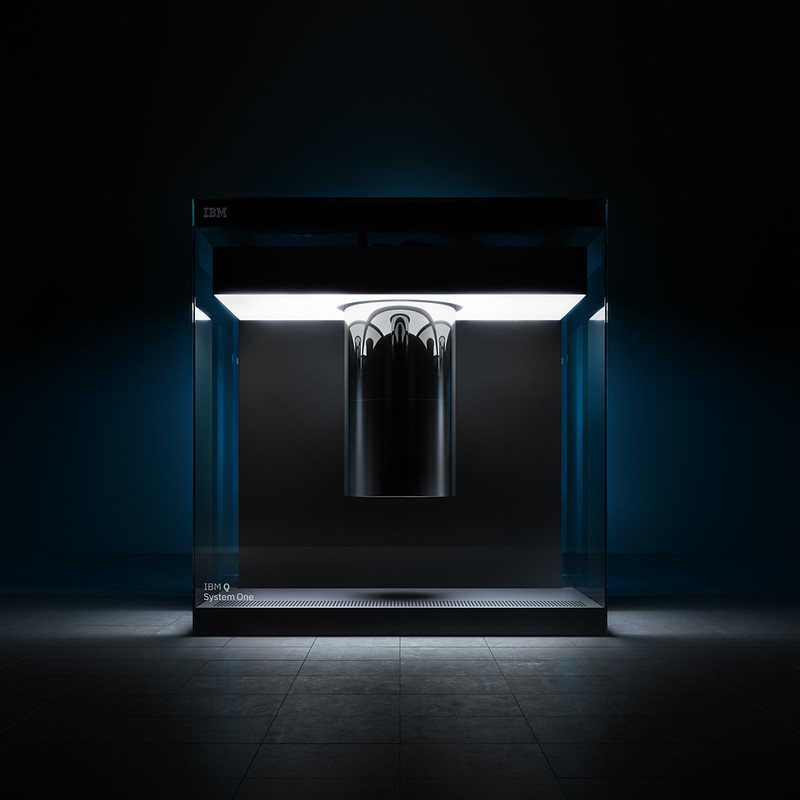
\includegraphics[width=.9\linewidth]{./assets/sysone.jpg}
\caption{\textbf{IBM System One}}
\end{figure}

\begin{quote}
``By augmenting human performance, AI has the potential to markedly improve productivity, efficiency, workflow, accuracy and speed, both for [physicians] and for patients … What I’m most excited about is using the future to bring back the past: to restore the care in healthcare.'' . \mbox{--- Eric Topol}
\end{quote}

\section{Introduction}
\label{sec:org3746fb1}

Healthcare data—such as information from clinical trials, disease registries, electronic health records (EHRs), and medical devices—is growing at a compound annual growth rate of 36 percent  . Increasingly, this data helps address 4 challenges associated with healthcare:

\begin{itemize}
\item Better health
\item Lower cost
\item Enhanced patient experiences
\item Improved healthcare practitioner work lives.
\end{itemize}

At the same time, healthcare consumers are making more decisions and have to navigate an increasingly complex system. Traditionally, diagnosing a patient’s condition has been based heavily on the umbrella approach, which is based solely on the patient-reported symptoms, resulting in an umbrella diagnosis and treatment that frequently fails to achieve their intended effects due to individual variability. As a result, many existing therapies fail to achieve their intended effects due to individual variability. Precision medicine aims to allow tailor prevention and treatment with an individual approach. Due to the complexity of human biology, individualized medicine requires taking into account aspects that go well beyond standard medical care. Medical care only has a relative contribution of 10 to 20 percent to outcomes; health-related behaviors, socioeconomic factors, and environmental aspects account for the other 80 to 90 percent. Computationally, the interdependencies and correlations among these diverse contributors create formidable challenges concerning optimizing treatment effectiveness.

Significant investments are being made to deliver the right data and powerful insights at the point of care. Industry incumbents and new entrants alike are trying to create digital experiences that reinforce healthy, preventive behaviors. Despite that, accounting for the exponential possibilities from this diversity of new data is stretching the capabilities of classical computing systems. [\citeprocitem{1}{Grumbling and Horowitz 2020}].

\section{AI in Precision Medicine}
\label{sec:orgaa38e6b}

\begin{figure}[htbp]
\centering
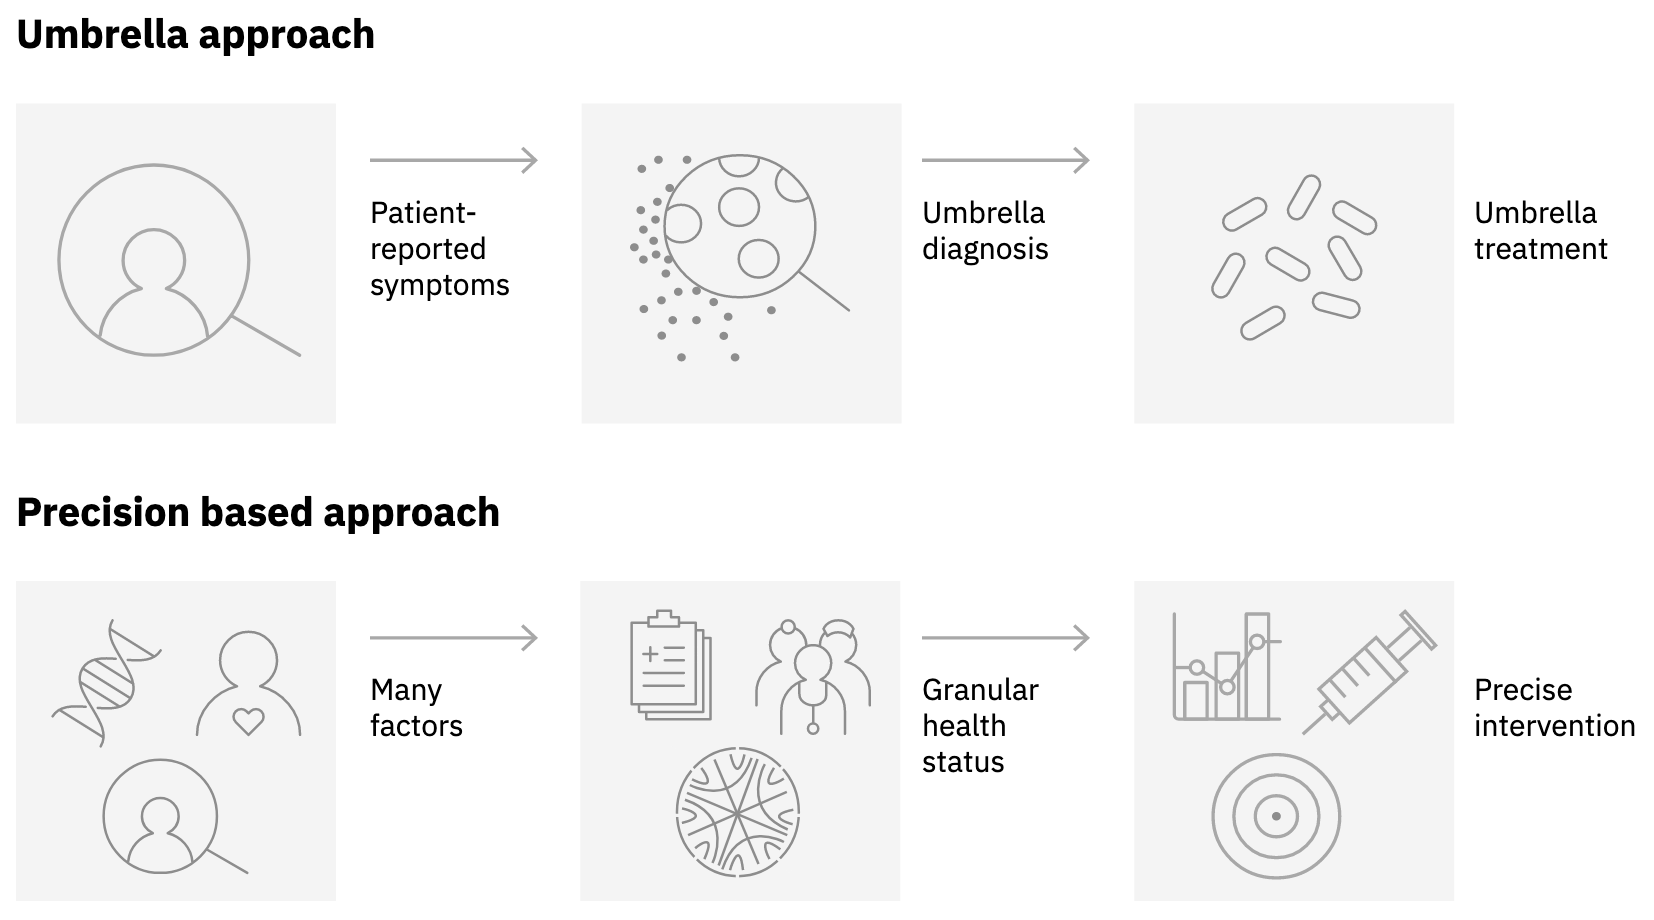
\includegraphics[width=.9\linewidth]{./assets/precisionMedicineApproach.png}
\caption{\textbf{Precision Approach vs. Umbrella Approach}}
\end{figure}

A key aspect of tailoring medical approaches is proactivity. Early treatments and preventive interventions tend to drastically improve outcomes and optimize costs. Classical machine learning has already shown some promise in predicting the risk of future diseases for a range of patient groups based on EHRs. Supervised and unsupervised quantum-enhanced machine learning techniques could allow earlier more accurate, and more granular risk predictions. Eventually, medical practitioners might even have the tools to understand how an individual’s risk for any given condition changes over time, enabled by continual virtual diagnostics based on ongoing data streams from individuals.

\subsection{Accelerating AI with Quantum Computing}
\label{sec:org5f9b1a5}

Quantum computers process information in a fundamentally different way from traditional computers. Previous computer technology advancements—such as integrated circuits—enabled faster computing, but were still based on classical information processing. These computers manipulate quantum bits (qubits). These are unlike classical bits, which store information as either a 0 or 1, and they can display uniquely quantum properties, such as entanglement. As a result, it becomes possible to construct quantum algorithms that can outperform their classical counterparts which are not able to leverage quantum phenomena.

\begin{itemize}
\item Chemistry, machine learning/artificial intelligence (AI), optimization, or simulation tasks. Machine learning has shown potential to be enhanced by quantum computing and is symbiotically helping drive quantum advances
\item Complex correlations and interdependencies among many highly interconnected elements, such as molecular structures in which many electrons interact
\item Inherent scaling limits of relevant classical algorithms. For instance, the resource requirements of classical algorithms may increase exponentially with problem size, as is the case when simulating the time evolution of quantum systems.
\end{itemize}

\subsection{Hybrid Quantum-Classical Neural Networks}
\label{sec:org4513971}

\begin{figure}[htbp]
\centering
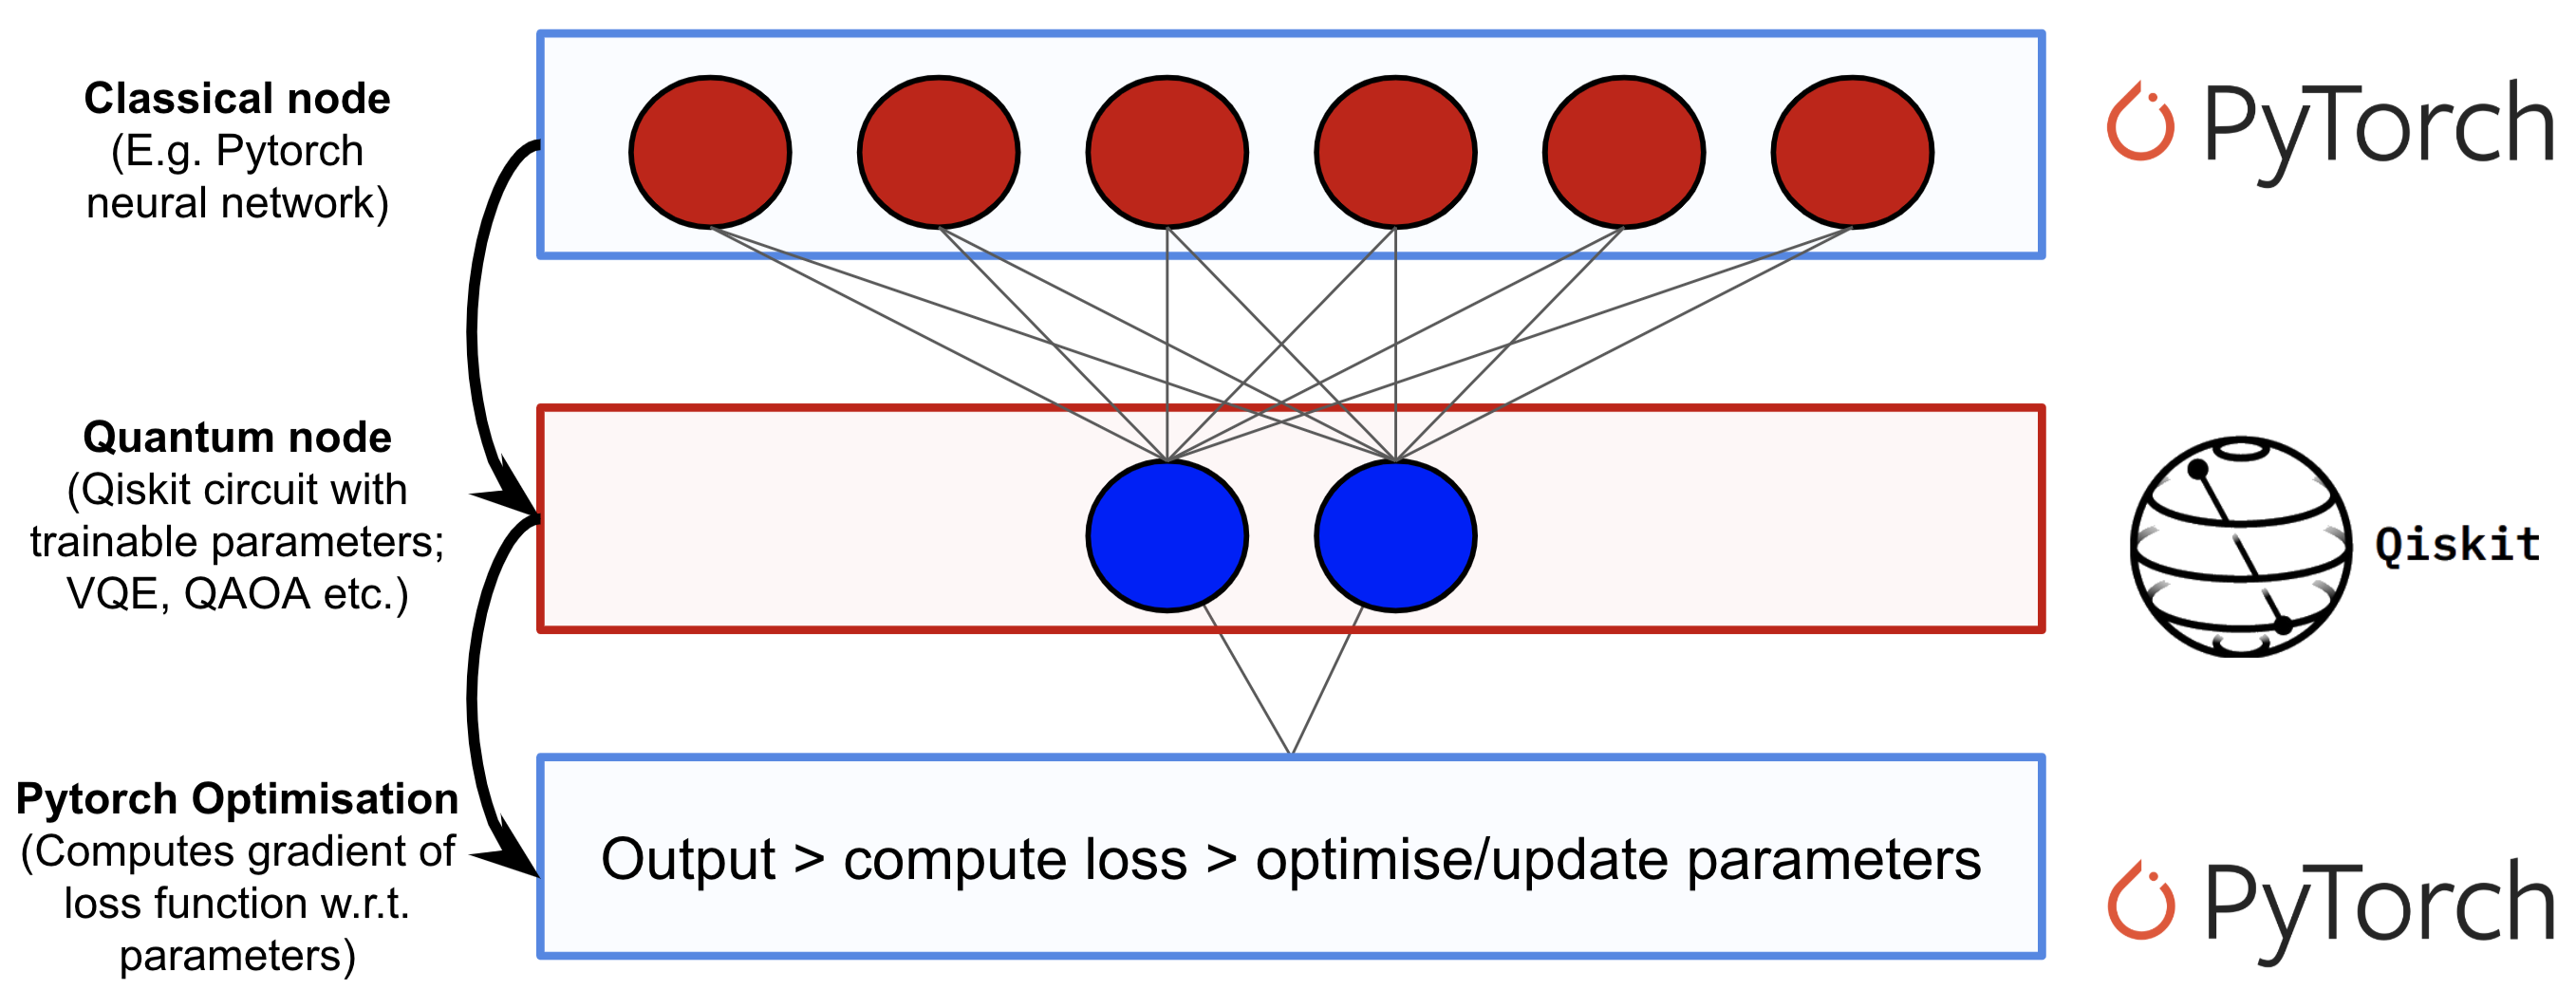
\includegraphics[width=.9\linewidth]{./assets/hybridnetwork.png}
\caption{\textbf{Example of a Hybrid Quantum-Classical Neural Network}}
\end{figure}

The most computationally demanding part of gradient-based algorithms, namely, computing the fitness function and its gradient for control input, can be accomplished by the process of evolution and measurement on quantum hardware. By posing queries to and receiving answers from these devices, classical computing devices update the control parameters until an optimal control solution is found.

Using this hybrid approach gives rise to interesting areas of research that seek to leverage the principles of quantum mechanics to augment machine learning or vice-versa. Enabling us to enhance classical ML algorithms by outsourcing difficult calculations to a quantum computer.

To create a quantum-classical neural network, one can implement a hidden layer for a neural network using a parameterized quantum circuit, a quantum circuit where the rotation angles for each gate are specified by the components of a classical input vector. The outputs from the neural network's previous layer will be collected and used as the inputs for a parameterized circuit. The measurement statistics of the circuit can then be collected and used as inputs for the following layer.

In this example, \(\sigma\) is a nonlinear function and \(h_{i}\) is the value of neuron i at each hidden layer. \(R(h_{i})\) represents any rotation gate about an angle equal to \(h_{i}\) and \(y\) is the final prediction value generated from the hybrid network

\begin{figure}[htbp]
\centering
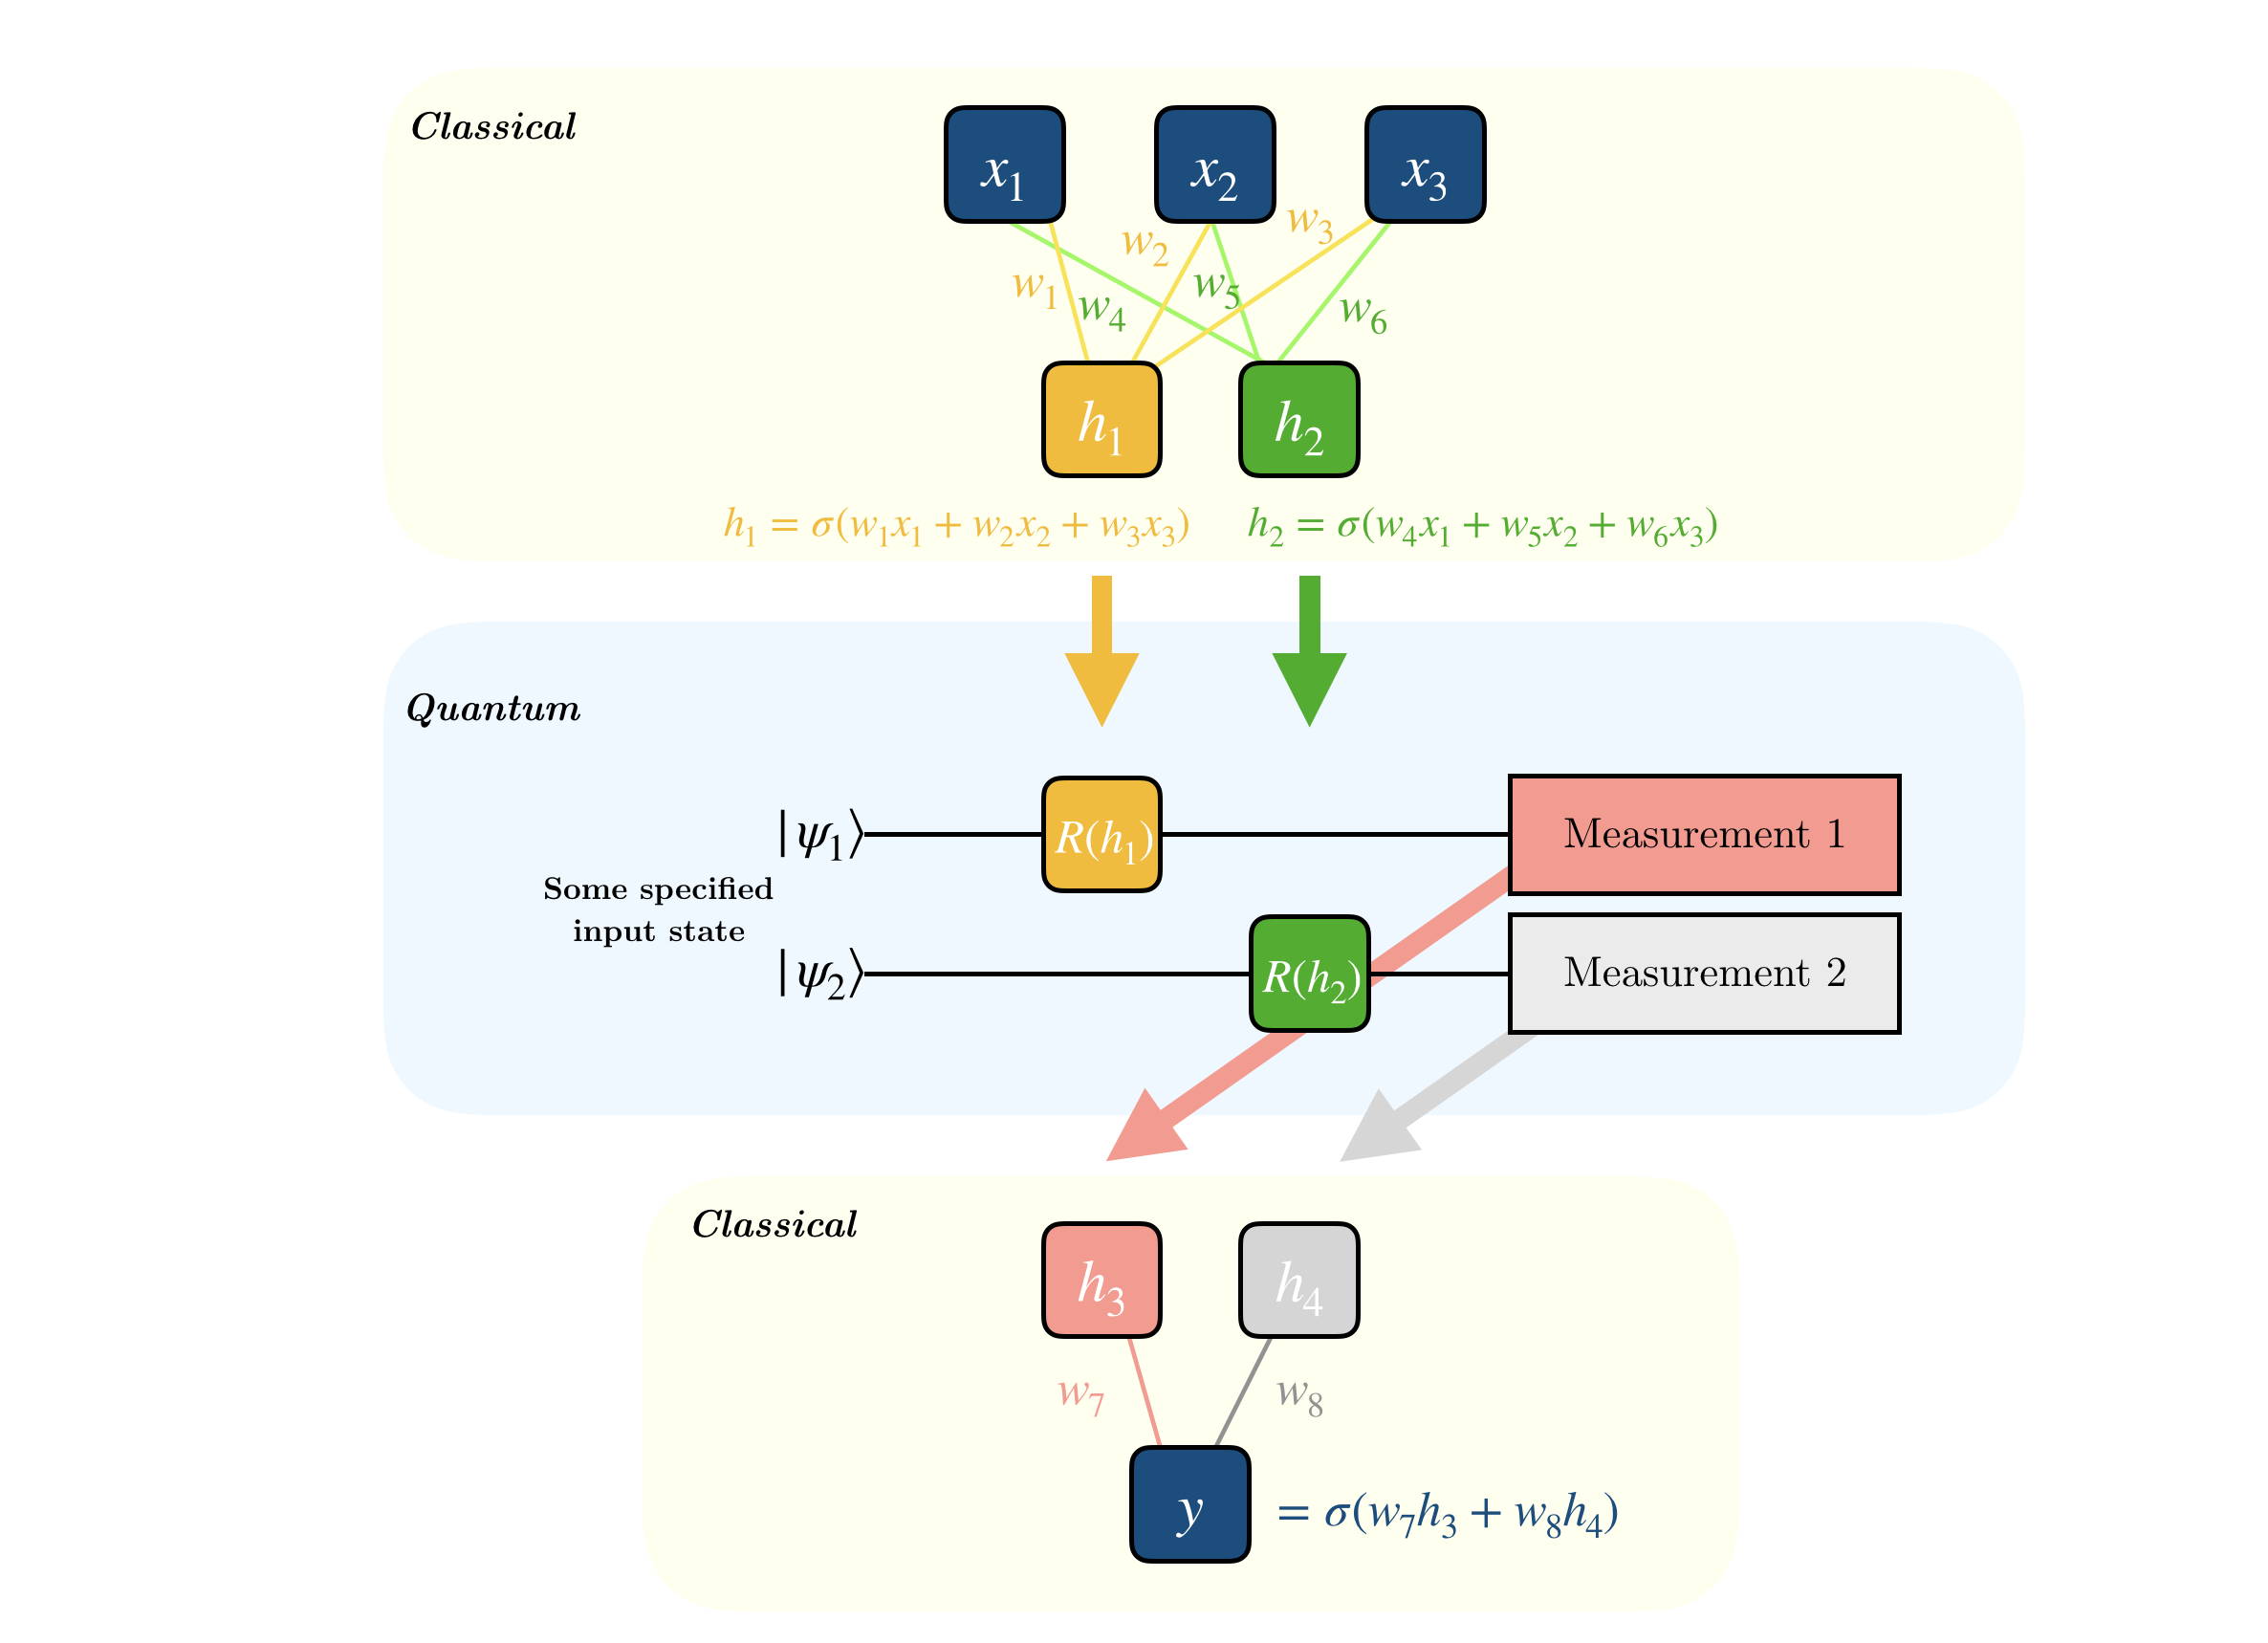
\includegraphics[width=.9\linewidth]{./assets/neuralnetworkQC.png}
\caption{\textbf{Quantum-classical Neural Network using a Parameterized Quantum Circuit}}
\end{figure}

\subsection{Generative Adversarial Networks}
\label{sec:org4a73d5d}

Generative Adversarial Networks, or GANs for short, are an approach to generative modeling using deep learning methods, such as convolutional neural networks. Generative modeling is an unsupervised learning task in machine learning that involves automatically discovering and learning the regularities or patterns in input data in such a way that the model can be used to generate or output new examples that plausibly could have been drawn from the original dataset.

GANs are a clever way of training a generative model by framing the problem as a supervised learning problem with two sub-models: the generator model that we train to generate new examples, and the discriminator model that tries to classify examples as either real (from the domain) or fake (generated). The two models are trained together in a zero-sum game, adversarial, until the discriminator model is fooled about half the time, meaning the generator model is generating plausible examples.

\subsubsection{MolGAN}
\label{sec:org6af9af7}

Existing drug discovery pipelines take 5-10 years and cost billions of dollars. Computational approaches aim to sample from regions of the whole molecular and solid-state compounds called chemical space which could be on the order of 1060. Deep generative models can model the underlying probability distribution of both the physical structures and property of drugs and relate them nonlinearly. By exploiting patterns in massive datasets, these models can distill salient features that characterize the molecules. We can utilize Generative Adversarial Networks (GANs) discover drug candidates by generating molecular structures that obey chemical and physical properties and show affinity towards binding with the receptor for a target disease.

Currently, this is accomplished through the Tensorflow library \href{https://github.com/nicola-decao/MolGAN}{MolGAN}. However,  However, classical GANs cannot explore certain regions of the chemical space and suffer from curse-of-dimensionality. Computing these drug candidates can be computationally expensive, and the resource requirements of these classical algorithms increase exponentially with problem size. On the other hand. A full quantum GAN may require more than 90 qubits even to generate QM9-like small molecules, and is impractical in the current day and age

\subsubsection{Qubit-efficient Quantum Molecule Generation}
\label{sec:org3384f98}

Once again, we can apply our hybrid approach. A qubit-efficient quantum GAN with a hybrid generator (QGAN-HG) can be used to learn a richer representation of molecules via searching exponentially large chemical space with fewer qubits and more efficiently than a classical GAN. The QGAN-HG model is composed of a hybrid quantum generator that supports various number of qubits and quantum circuit layers, and, a classical discriminator. The approach is significantly quicker than our classical GAN model.

\begin{center}
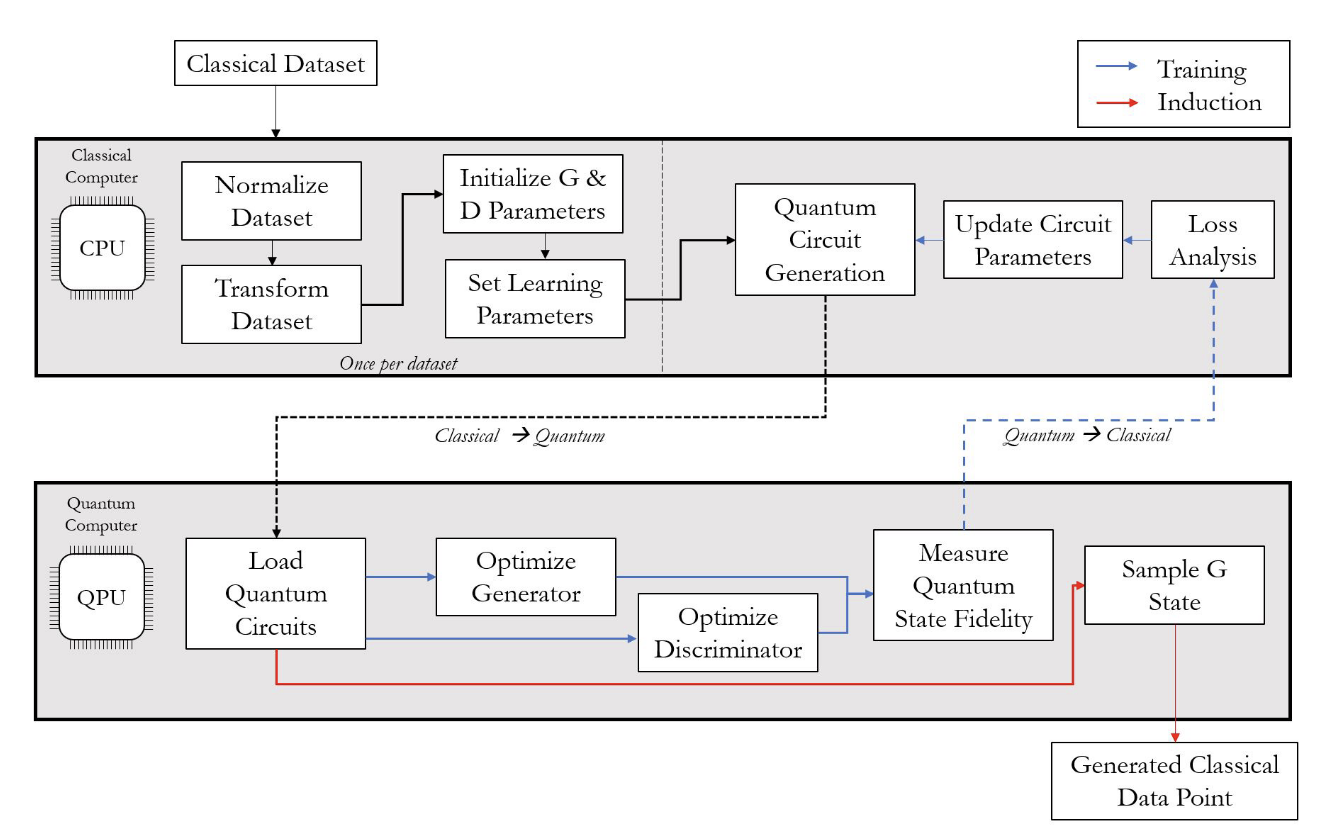
\includegraphics[width=.9\linewidth]{./assets/systemarchitecture.png}
\end{center}

\section{Prototype}
\label{sec:orgc2eb20e}

To test the speed, practicality, efficiency, and cost of quantum-accelerated ML as well as its usefulness in precision medicine, we have devised two prototypes written in Python. The concise, expressive, and dynamic nature of the Python language makes it well suited for prototyping tasks. Notebook one will test how viable our QML approach is at accelerating image and text sorting. This script can be adapted to identify mutations, distinguish genomic variants, as well as identify an indivudual's susceptiblity to rare diseases through an analysis of their previous health and history. Notebook 2 will generate viable drugs based on ones that currently exist, and will test how viable our QML approach is to accelerating current conventional drug discovery pipelines. Both models utilize PyTrorch and IBM's Quantum Services for training and testing

The full code for both notebooks are available under \href{prototype/}{the prototype folder}.

\subsection{Image recognition (QuTorch-HG)}
\label{sec:orgb83bbdc}

\begin{figure}[htbp]
\centering
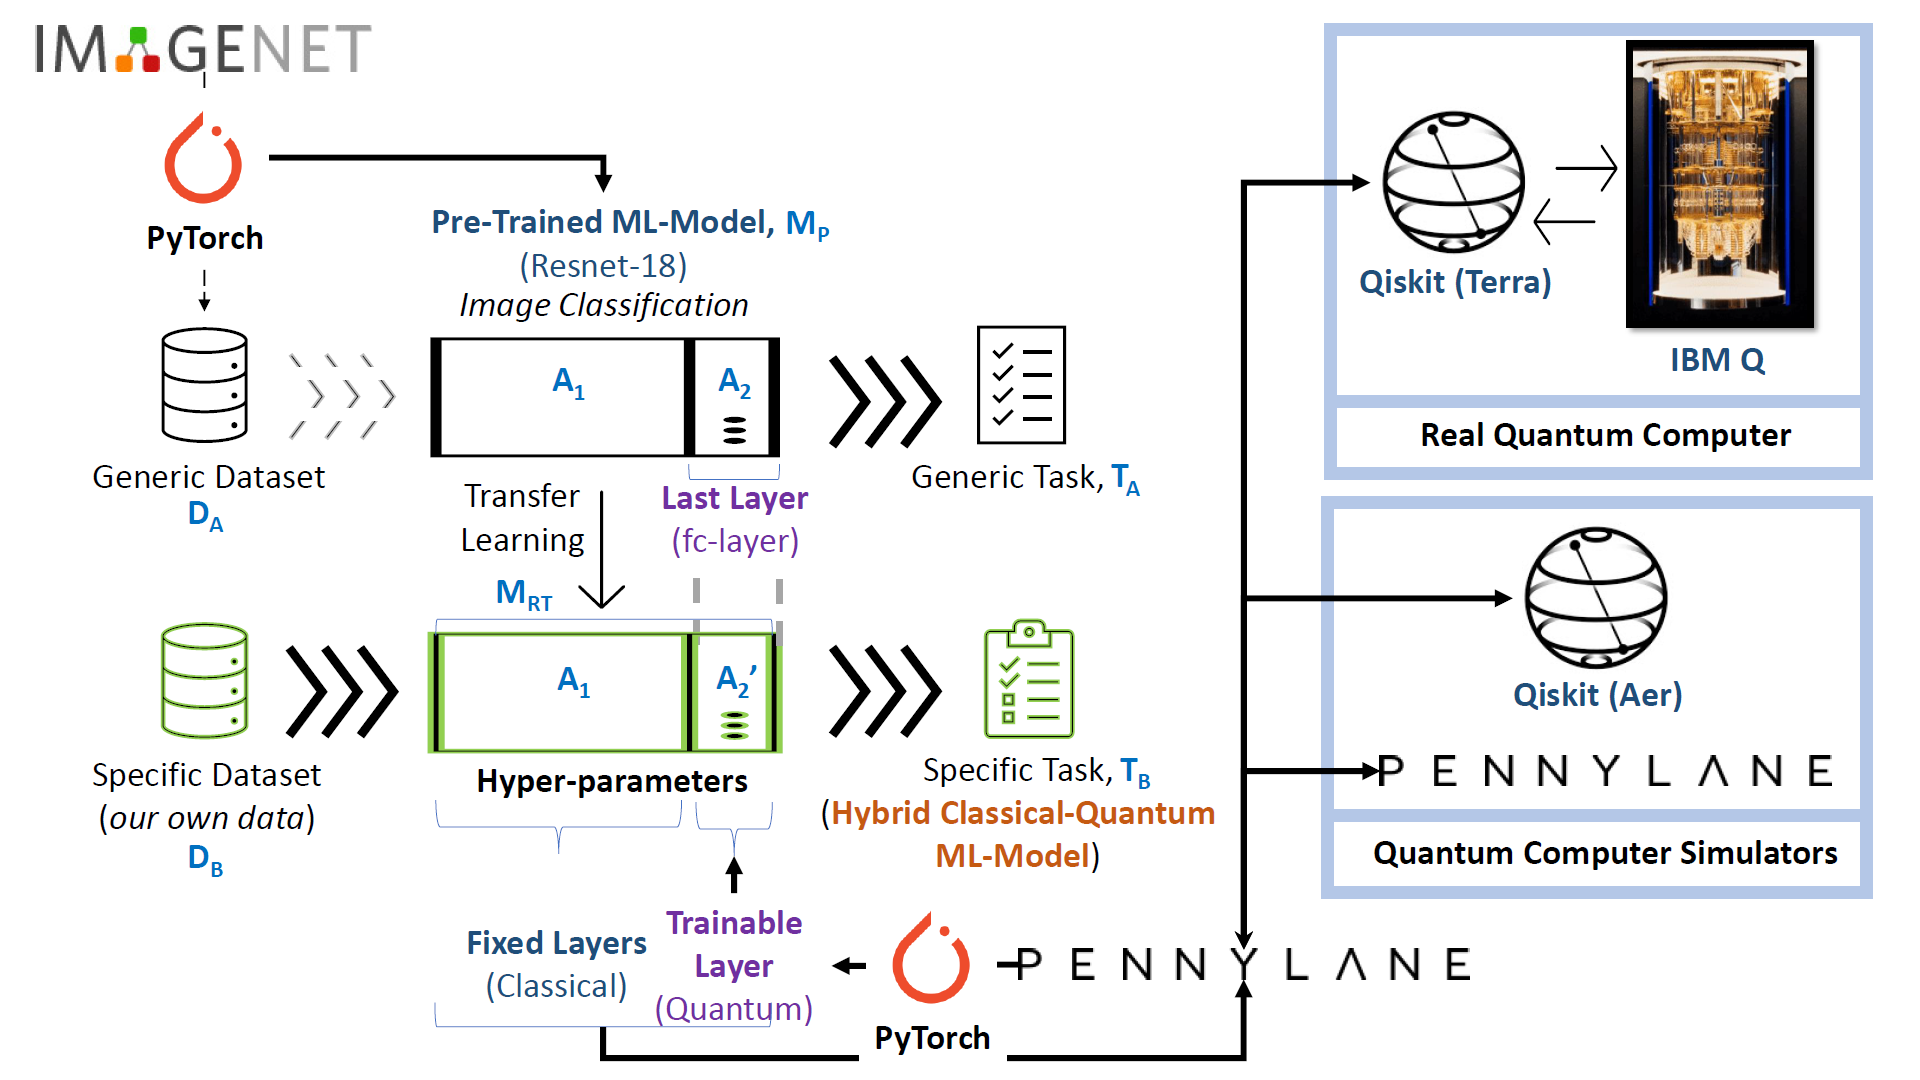
\includegraphics[width=.9\linewidth]{./assets/imagenet.png}
\caption{\textbf{Hybrid Base Nueral Network}}
\end{figure}

We have created a base neural network model, which utilizes hybrid machine learning to create a model trained from any dataset in ImageNet format. The base model is used as the base for Transfer Learning, on an Image Classification task (based on resnet18). The last layer of this pre-trained model (fully-connected/fc layer) is then modified through a quantum machine learning framework, generating a new model. We will be testing its efficiency, practicality, and accuracy. We are training the model with 4 Qubits at 8 epochs.

\subsection{Quantum Accelerated Drug \& Molecule Generation (QGAN-HG)}
\label{sec:org76ff07f}

\begin{figure}[htbp]
\centering
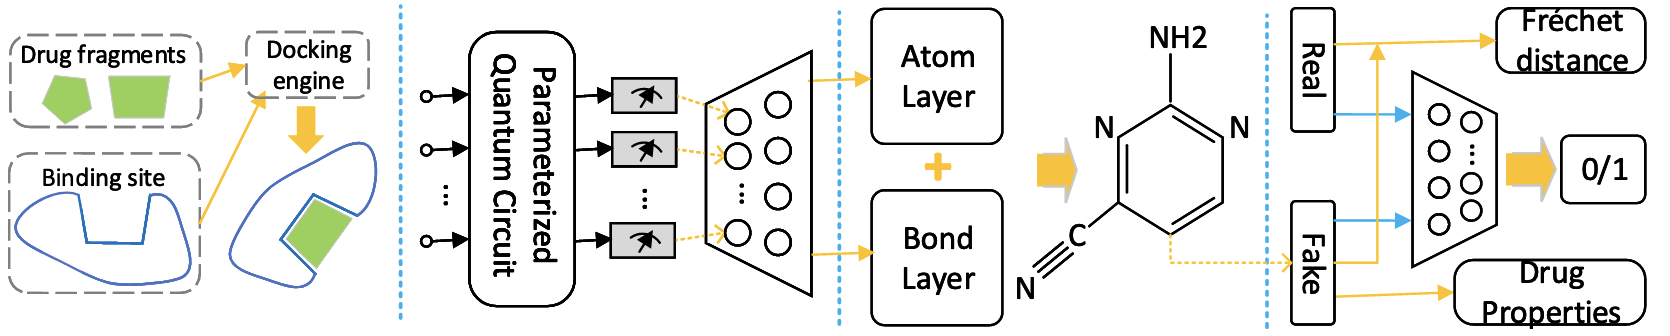
\includegraphics[width=.9\linewidth]{./assets/quganflow.png}
\caption{\textbf{Quantum Accelerated Molecule Generation}}
\end{figure}

Firstly, only generated molecules that have high affinity towards the receptor binding sites are considered as valid. Next, a parameterized quantum circuit with last-layer N measures the expectation values and a processes it through a classical stage. Then, we apply the atom layer and bond layer to generate synthetic molecular graphs. Afterwards, a batch of real molecules from a training dataset (in this case we are using QM9) and a batch of generated synthetic molecules are fed into a classical discriminator for real/synthetic prediction and Frechet distance score calculation.

\subsection{Data}
\label{sec:org25dde5d}

Our Image Data is obtained from Standford's ImageNet collection, a large-scale ontology of images built upon the WordNet structure. ImageNet aims to populate the majority of the 80,000 synsets of WordNet with an average of 500–1000 clean and full resolution images, with currently over 14,197,122 images and 21841 synsets indexed. The specific dataset used in this example can be found at \href{https://www.kaggle.com/paultimothymooney/chest-xray-pneumonia}{Paul Timothy: Chest X-RAY Pneumonia Dataset}, and is liscensed under CC0 1.0: Public Domain.

The Molecular data used to train our MolGAN and QuGAN models is the QM9 Dataset obtained from Anatole von Lilienfeld. The dataset contains the computed geometric, energetic, electronic, and thermodynamic properties for 134k stable small organic molecules made up of CHONF. These molecules correspond to the subset of all 133,885 species with up to nine heavy atoms (CONF) out of the GDB-17 chemical universe of 166 billion organic molecules. The model is trained on geometries, corresponding harmonic frequencies, dipole moments, polarizabilities, along with energies and enthalpies. The dataset is hosted on \href{https://doi.org/10.6084/m9.figshare.c.978904.v5}{figshare}.

\subsection{Tools and Hardware}
\label{sec:orgdbffe93}

The open-source Qiskit framework provides convenient access to multiple quantum simulators as well as a real quantum computer backend. The user can choose to utilize either IBM's cloud-based QASM simulator technology, Google's local equivalent Cirq, and Pennylane's quicker but less accurate lightning simulator. All three backends allow for quick training and testing via quantum simulators and real quantum hardware.

\begin{figure}[htbp]
\centering
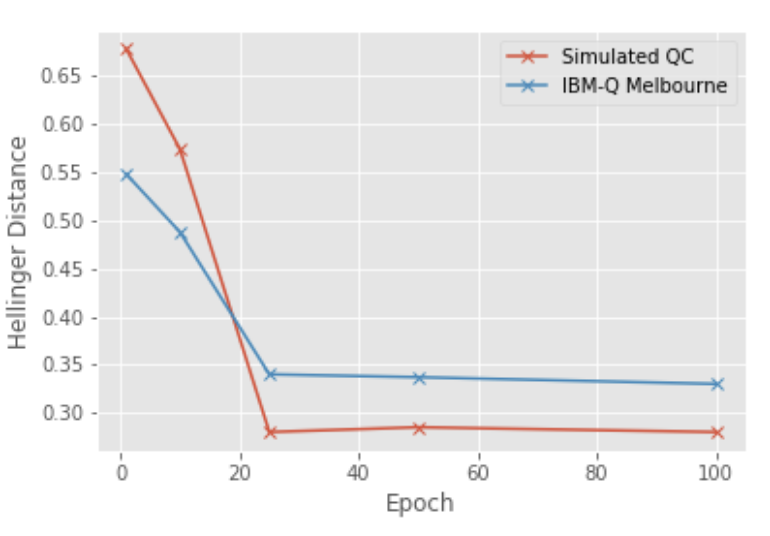
\includegraphics[width=250pt]{./assets/simulatedvsreal.png}
\caption{\textbf{Actual vs. Simulated Hardware}}
\end{figure}

While simulated hardware produces \emph{slightly} different results to actual hardware, the margin is within 1\%. The tests below were conducted using actual IBMQ hardware, on the \verb~ibmq_lima~ quantum computer [\citeprocitem{2}{Quantum 2021}]

Code is developed in Jupyter notebooks allowing for quick prototypng, and utilize PyTorch for pre-processing and post-processing of our neural network, taking advantage of GPU Acceleration via Nvidia CUDA if available. This allows us to process images in realtime on Google's Compute Engine VM's via Google Colab, allowing for low operating costs, high performance, and good portability.

\begin{figure}[htbp]
\centering

\includegraphics[width=.9\linewidth]{./assets/circuit.png}
\caption{\textbf{Sample Generated Quantum Circuit on IBMQ}}
\end{figure}

\section{Results}
\label{sec:orga8ccec7}

\subsection{Speed}
\label{sec:orgfc5ab1f}

This is the largest benefit of quantum-accelerated machine learning.  We can see that in both algorithms, quantum computing provided an exponential increase in speed over the non-accelerated counterpart. In the case of QGAN, We can see anywhere from a 8-32\% decrease in the time needed to generate molecules, with the same input parameters. In the case of our QuTorch-HG algorithm, it can process a batch of images within 1/10th of a second, allowing for models to be trained at 95\% accuracy in under 5 minutes! A similar model, written with tensorflow and trained on the same cpu, took 32 minutes to achieve 94.3\% accuracy.

\begin{figure}[htbp]
\centering
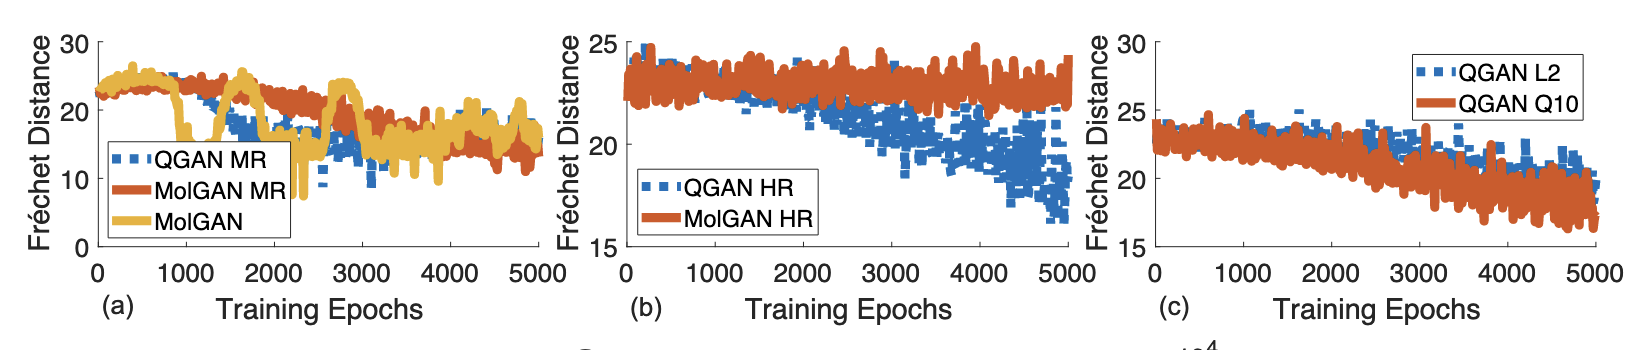
\includegraphics[width=.9\linewidth]{./assets/quganresults.png}
\caption{\textbf{Training comparison among GAN flavors}}
\end{figure}

\subsection{Accuracy}
\label{sec:org8b71621}

In both prototypes, accuracy was as expected. The QuTorch-HG algorithm tested at around 96.23\% accuracy on average on average after 8 epochs. The QGAN prototype created valid molecules 100\% of the time during our testing.

\begin{figure}[htbp]
\centering
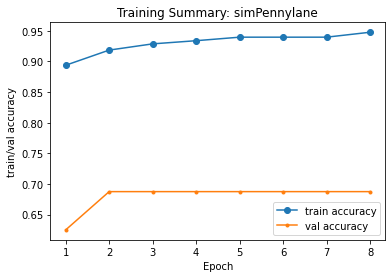
\includegraphics[width=250pt]{./assets/output1.png}
\caption{\textbf{Training Accuracy vs. Epochs}}
\end{figure}
\begin{figure}[htbp]
\centering
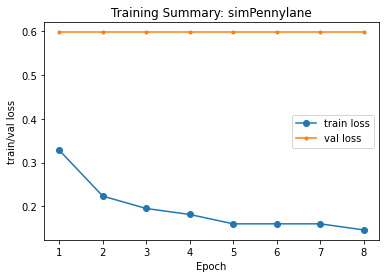
\includegraphics[width=250pt]{./assets/output2.png}
\caption{\textbf{Training Accuracy vs. Epochs}}
\end{figure}

\begin{figure}[htbp]
\centering
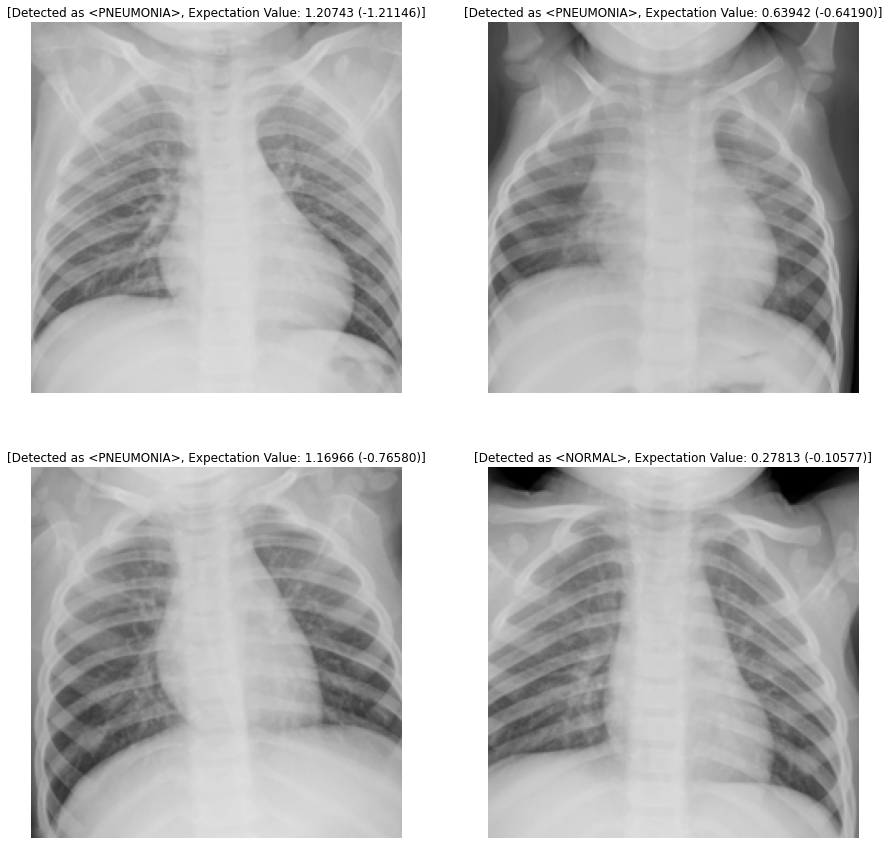
\includegraphics[width=250pt]{./assets/output3.png}
\caption{\textbf{Analysis of Pneumonia through our QuTorch-HG algorithm}}
\end{figure}

\begin{figure}[htbp]
\centering
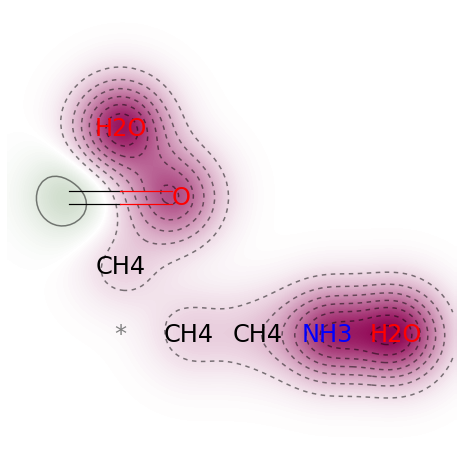
\includegraphics[width=250pt]{./assets/output4.png}
\caption{\textbf{Sample Generated Molecule through our QGAN-HG algorithm}}
\end{figure}

\subsection{Pricing}
\label{sec:org2502bef}

As of early 2022, IBM Quantum Services allows researchers and students to use their 5 qubit quantum computers for development free of charge. The GPU accelerator was provided by Google's Colab program, free of charge as well. Those looking for real-time analysis can utilize Google Compute Engine VM's, such as the A2 Accelerator for just \$0.009 an hour. Our hybrid model is effecient and as all computation is handled through the cloud, energy costs are nominal.

On the other hand our algorithms can also be applied to healthcare cost analysis, such as improving insurance pricing computations, allowing for lower average premiums, as well as better-tailored premium options. We strongly believe investing in quantum computing now will result in increased profits in the future.

\section{Conclusion and Further Research}
\label{sec:org1f114d9}

\section{References}
\label{sec:orgddb3177}

\begin{hangparas}{1.5em}{1}
\hypertarget{citeproc_bib_item_1}{\textsc{Grumbling, E. and Horowitz, M.} 2020. \href{https://doi.org/10.17226/25196}{Quantum computing}. .}

\hypertarget{citeproc_bib_item_2}{\textsc{Quantum, I.} 2021. \href{https://quantum-computing.ibm.com/}{Ibm quantum services}. .}
\end{hangparas}

\begin{quote}
We acknowledge the use of IBM Quantum services for this work. The views expressed are those of the authors, and do not reflect the official policy or position of IBM or the IBM Quantum team.
\end{quote}
\end{document}
